\documentclass{beamer}
\usetheme{Frankfurt}
\usepackage[utf8]{inputenc}
\usepackage{amsmath, kotex, graphicx}

\title{Oxygen Reduction Reaction}
\subtitle{ORR on Macrocyclic Transition Metal Complexes and Catalyses}
\author[16-087 이현동]
{16-087 이현동\inst{1}}
\institute
{
  \inst{1}%
  Korea Science Academy of KAIST
}
\date{May 06, 2017}

\begin{document}
\begin{frame}
\titlepage
\end{frame}

\section{ORR on Macrocyclic Transition Metal Complexes}

\begin{frame}
\frametitle{Outline}
\tableofcontents[currentsection]
\end{frame}

% ################################################## 

\subsection{Catalysis by Transition Metal Macrocyclic Complexes}

\begin{frame}
\frametitle{Catalysis by Transition Metal Macrocyclic Complexes}

\begin{block}{Transition Metal Macrocyclic Complexes}
\begin{itemize}
\item{Catalyzes ORR, making H$_2$O$_2$ or H$_2$O in the electron path\\ (Through either 2- or 4-electron path)}
\item{Sometimes they catalyze 1-electron ORR, making superoxides)}
\end{itemize}
\end{block}

\begin{block}{Catalytic Reaction Mechanism}
\begin{enumerate}
    \item{Oxygen-Metal ion center compound}
    \item{Electron transfer from metal to oxygen}
    \item{Increased proton from electrolyte $\longrightarrow$ Production of H$_2$O$_2$}
    \item{Further reduction of H$_2$O$_2$ to H$_2$O, or final product}
\end{enumerate}
\end{block}
\end{frame}

\begin{frame}
\begin{figure}[htbp]
    \begin{center}
    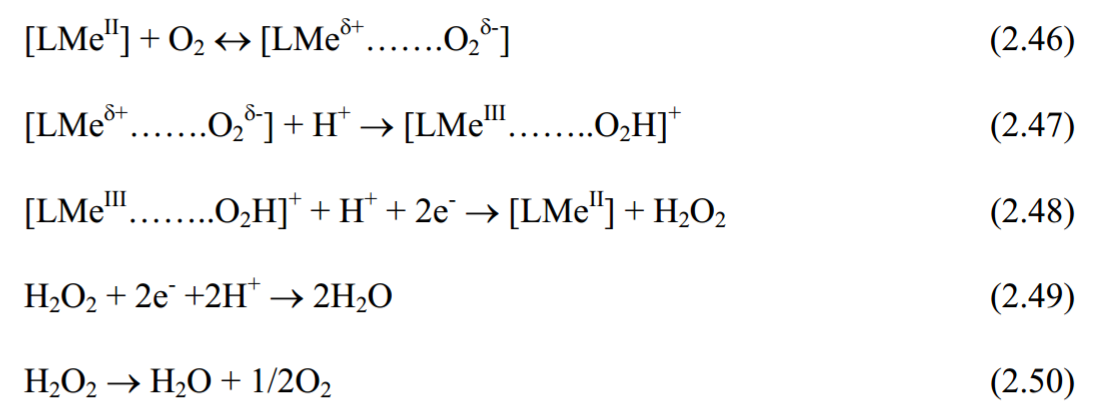
\includegraphics[scale=0.65]{image1}
    \caption{Catalytic reaction mechanism of metal compound}
    \end{center}
\end{figure}
\begin{itemize}
\item{'L' means ligands and 'Me' is metal center}
\end{itemize}
\end{frame}

% ######################################################

\subsection{Transition Metal Macrocycles as ORR Catalysts}
\subsubsection{Metal Centers and the Ligand Effect on ORR Activity}
% %%%%%%%%%%%%%%%%%%%%%%%%%%%%%%%%%%%%%%%%%%%%%%%%%%%%%%%

\begin{frame}
\frametitle{Metal Centers and the Ligand Effect on ORR Activity}
\begin{block}{Transition Metal Macrocyclic Compounds}
Its catalytic acvitity depends on the following:
\begin{itemize}
\item{Individual transition metal center}
\item{Macrocyclic ligands}
\item{Size of $\pi$ electron system}
\end{itemize}
\end{block}

\begin{exampleblock}{Type of Compound Elements}
\begin{itemize}
    \item{The activity changes with respect to the central metal ions: Fe$>$Co$>$Ni$>$Cu}
    \item{Fe:\emph{ N$_4>$}N$_2$O$_2>$N$_2$S$_2>$O$_4=$S$_4$ (inactive)}
    \item{Co: N$_2$O$_2>$\emph{N$_4>$}N$_2$S$_2>$O$_4=$S$_4$}
    \item{Ni: O$_4>$N$_2$O$_2$>N$_2>$S$_2>$N$_4$}
    \item{Cu: N$_4$>O$_4>$N$_2$O$_2>$N$_2$S$_1>$S$_4$ (inactive)}
\end{itemize}
\end{exampleblock}
\end{frame}

\subsubsection{M-N$_4$ ORR Catalysts}
% %%%%%%%%%%%%%%%%%%%%%%%%%%%%%%%%%%%%%%%%%%%%%%%%% 
\begin{frame}
\frametitle{M-N$_4$ ORR Catalysts}
\begin{block}{M-N$_4$ Complex}

\begin{itemize}
\item{Strong and irreversible adsorption on graphite electrode surface}
\item{Form a monolayer or multilayers of ORR catalysts}
\item[$\rightarrow$]{ Form a well-defined electrode surface}
\end{itemize}
\end{block}
\end{frame}

% %%%%%%%%%%%%%%%%%%%%%%%%%%%%%%%%%%%%%%%%%%%%%%%%%%%%%
\begin{frame}
\frametitle{Fe-N$_4$ ORR Catalyst}
\begin{block}{Fe-N$_4$ ORR Catalyst}

\begin{itemize}
\item{Usually 4-electron transfer path, producing H$_2$O}
\item{ORR catalysis by Fe tetrakis (4-N-methylpyridyl) porphyrin $\longrightarrow$ mixture of H$_2$O and H$_2$O$_2$ }
\item{Fe porphyrins (FeTPP and FePPIX): Catalyze 4-electron ORR}
\item{FeTPyP: Catalyzes 2-electron ORR}
\item{\emph{In most cases, Fe-N$_4$ catalyzes 4-electron ORR and doesn't produce H$_2$O}}
\end{itemize}

\end{block}
\end{frame}
% %%%%%%%%%%%%%%%%%%%%%%%%%%%%%%%%%%%%%%%%%%%%%%%%%%%%%%%%%%%
\begin{frame}
\frametitle{Co-N$_4$ ORR Catalyst}
\begin{block}{Co-N$_4$ ORR Catalyst}

\begin{itemize}
\item{Mononuclear Co-N$_4$ complex: Catalyze only 2-electron ORR}
\item{Bi-nuclear Co-N$_4$ complexes or Co-N$_4$ dimers: \newline Catalyze both 2- and 4-electron ORR}
\item{Planar bicobalt complex $(ex. (Co_2TAPH)^{4+})$: 4-electron ORR in alkaline}
\end{itemize}

\end{block}

\begin{figure}[htbp]
    \begin{center}
    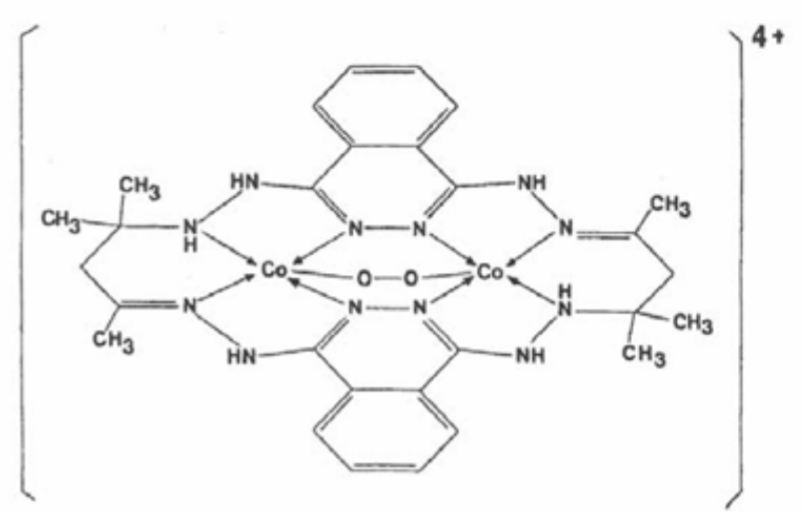
\includegraphics[scale=0.35]{image2}
    \caption {Dimetal complex $(Co_2TAPH)^{4+}(NO_3)_4$}
    \end{center}
\end{figure}

\end{frame}
% %%%%%%%%%%%%%%%%%%%%%%%%%%%%%%%%%%%%%%%%%%%%%%%%%%%%%%%%%%%% 
\begin{frame}
\frametitle{Co-N$_4$ ORR Catalyst}
\begin{itemize}
\item{Interaction between O$_2$ and the Co metal centers}
\item{Effectively weaken the O-O bond, making it break easily}
\newline
\item{Face-to face di-Co-N$_4$ complexes}
\end{itemize}

\begin{figure}[htbp]
    \begin{center}
    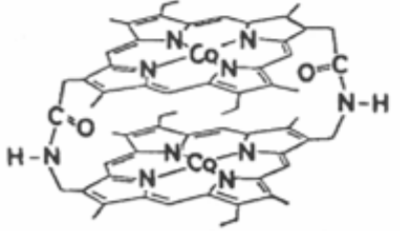
\includegraphics[scale=1]{image3}
    \caption{Face-to-face Co-Co 4-porphyrin}
    \end{center}
\end{figure}
\end{frame}
% %%%%%%%%%%%%%%%%%%%%%%%%%%%%%%%%%%%%%%%%%%%%%%%%

\begin{frame}
\frametitle{Co-N$_4$ ORR Catalyst}

\begin{itemize}
\item{Co-Co Distance around $4 \ \AA$: O-O Bridge $\longrightarrow$ 4-electron path}
\item{Co-Co Distance  $ >4 \ \AA $ or $<4 \ \AA$: 2-electron path (peroxide)}
\end{itemize}

\begin{figure}[htbp]
    \begin{center}
    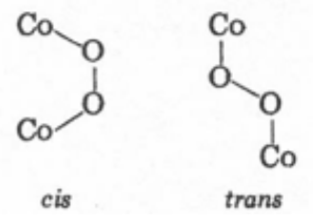
\includegraphics[scale=1]{image4}
    \caption{Cis- and trans-Co-O-O-Co facial configuration }
    \end{center}
\end{figure}
\end{frame}
% %%%%%%%%%%%%%%%%%%%%%%%%%%%%%%%%%%%%
\begin{frame}
\frametitle{Co Corroles Series}
\begin{itemize}
\item{Mixed valent Co(II)/Co(III) complexes: (PCY)Co$_2$, (BCY)Co$_2$}
\item{Catalyze the direct 4-electron pathway of ORR (O$_2$ to H$_2$O)}
\item{Path having \alert{anthracene spacer} is the most efficient \newline}
\item{0.47 V SCE for (PCA)Co$_2$ and 0.39 V for (BCA)Co$_2$}
\item{(Me$_4$Ph$_5$Cor)Co catalyze ORR at $E_{1/2} = 0.38$ V, final product H$_2$O$_2$ and H$_2$O}
\end{itemize}
\end{frame}
% %%%%%%%%%%%%%%%%%%%%
\begin{frame}
\frametitle{Macrocylic Rings and ORR Catalytic Activity}
\begin{itemize}
\item{Co-phthalocyanine complexes }
\end{itemize}
\end{frame}
% %%%%%%%%%%%%%%%%%%%%%%%%%%%%%%%%%%%%%%%%%%%%%%%%%%%%%
\subsubsection{Heat-treated Transition Metal Macrocyclic Complexes}
% %%%%%%%%%%%%%%%%%%%%%%%%%%%%%%%%%%%%%%%%%%
\begin{frame}
    \frametitle{Heat-treated Transition Metal Macrocyclic Complexes}
    \begin{block}{Transition Metal Macrocyclic Complexes and Heat-Treatment}
    \begin{itemize}
    \item{Usaully do not have long-term stability in concentrated acidic / alkaline solutions}
    \item{Thermal treatment after adsorbed on high-surface-area carbon support particle $\longrightarrow$ Increase stability and catalytic activity}
    \item{Another way: Heat-treating the macrocycles adsorbed on carbon substrates}
    \item{Phase change in transition metal macrocyclic complex: iron phthalocyanine $\alpha \longrightarrow \beta$}
    
    \end{itemize}
    
    \end{block}
\end{frame}
% %%%%%%%%%%%%%%%%%%%%%%
\subsection{ORR Kinetics Catalyzed by Transition Metal Macrocyclic Complexes}
% %%%%%%%%%%%%%%%%%%%%%
\begin{frame}{Kinetics of ORR; Catalyzed by Metal Comlex}
\begin{block}{Difference in Tafel Slope Values}
\begin{itemize}
\item{\alert{M-N$_4$ complexes} have different Tafel slopes, depending on catalysts used}
\item{\alert{CoTSP} catalyzes 2-electron ORR, producing H$_2$O$_2$. It has Tafel slope values of 120, 135, 155 mV/dec}
\item{\alert{Dicobalt porphyrin dimers} had Tafel slope of 65mv/dec}
\item{\alert{Fe-N$_4$} has varying Tafel slope depending on pH}
\itemize{추가바람}


\end{itemize}
\end{block}
\end{frame}
% %%%%%%%%%%%%%%%%%%%%%%%%%%%%%%%%%%%%%
\section{ORR Catalyzed by Other Catalysts}
\subsection{ORR Catalyzed by Transition Metal Chalcogenides}
% %%%%%%%%%%%%%%%%%%%%%%%%%%%%%%%%%%%%%%%%%%%%%%%%%%%%
\begin{frame}
\frametitle{Outline}
\tableofcontents[currentsection]
\end{frame}
% %%%%%%%%%%%%%%%%%%%%%%%%%%%%%%%%%%%%%%%%%%%%%%%%%%%

\subsubsection{Chalcogenides and Oxygen Reduction Reaction Products}
\begin{frame}
\frametitle{Chalcogenides and Oxygen Reduction Reaction Products}

\begin{block}{Transition Metal Chalcogenides}
\begin{itemize}
\item{Group of materials that show catalytic activity towards ORR}
\item{\alert{Chevrel phase-type compounds} (Mo$_4$Ru$_2$Se$_8$) and \newline \alert{Amorphous phase compound} (Ru$_x$S$_y$) by the structure}
\item{Catalyze both 2- or 4- electron transfer depending on the catalyst used}
\end{itemize}
\end{block}

\begin{figure}[htbp]
    \begin{center}
    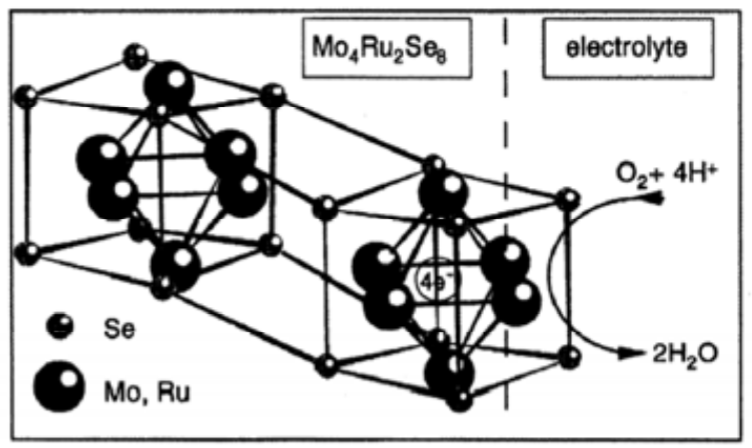
\includegraphics[scale=0.45]{image6}
    \caption{Mo$_4$Ru$_2$Se$_8$ and Interaction with Oxygen}
    \end{center}
\end{figure}
\end{frame}
% %%%%%%%%%%%%%%%%%%%%%%%%%%%%%%%%%%%%%%%%%%%%%%%%%%%
\subsubsection{Chalcogenide-catalyzed ORR Mechanism}
\begin{frame}{Chalcogenide-catalyzed ORR Mechanism}
     \begin{columns}[c] % contents are top vertically aligned
     \begin{column}[c]{5cm} % each column can also be its own environment
     \begin{block}{Property of Chalcogenides}
     
\begin{itemize}
\item{Semiconducting Property}
\item{Interaction of O$_2$ with the transition metal d-states originating from the mixed metal cluster}
\end{itemize}
\end{block}

     \end{column}
     \begin{column}[c]{5cm} % alternative top-align that's better for graphics
    
    
    \begin{figure}[htbp]
    \begin{center}
    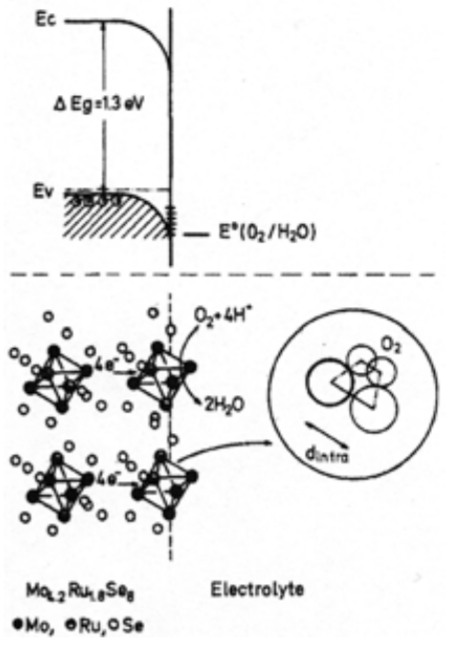
\includegraphics[scale=0.6]{image7}
    \caption{Mo$_4$Ru$_2$Se$_8$ and Interaction with Oxygen}
    \end{center}
\end{figure}


     \end{column}
     \end{columns}
\end{frame}
% %%%%%%%%%%%%%%%%%%%%%%%%%%%%%%%%%%%%%%%%%%%%%%%%%%%
\begin{frame}
\frametitle{Chalcogenide-catalyzed ORR Mechanism}

\begin{itemize}
\item{Energy gap between valence and conductance is \alert{1.3 eV}}
\item[$\longrightarrow$]{Characteristic of the compound as a degenerated p-type semiconductor}
\newline
\item{ORR starts when Fermi level of the electrode is 0.35 V above the O$_2$/H$_2$O redox potential}
\item[$\longrightarrow$]{O$_2$ interacts with transition metal atom through bridge-type bonding}
\item[$\longrightarrow$]{Metal distance increases, breaks the O-O bond and shift electronic level ($\because$ loss of the electron)}
\item[$\longrightarrow$]{15 \% cluster volume increase}
\end{itemize}
\end{frame}
% %%%%%%%%%%%%%%%%%%%%%%%%%%%%%%%%%%
\begin{frame}
\frametitle{Chalcogenide-catalyzed ORR Mechanism}
\begin{block}{Difference Between Chalcogenide and Pt Catalysis}
\begin{itemize}
\item{No stepwise, intermediate involving electron process}
\item{Involve synergistic multielectron transfer: Electrons dependent on each other}
\item{Positive feedback triggering subsequent loops: \newline Shown on the distance change between metal atoms}
\end{itemize}

\end{block}
\end{frame}
% %%%%%%%%%%%%%%%%%%%%%%%%%%%%%%%%%%%%%%%%%%%%%%%%%%%
\subsubsection{Kinetics of ORR Catalyzed by Chalcogenides}
\begin{frame}
\frametitle{Kinetics of ORR Catalyzed by Chalcogenides}

\begin{itemize}
\item{Can reach a level of 30–40 \% of the Pt catalyst activity}
\item{Tafel slope varies from 100 mV/dec up to 167 mV/dec}
\newline
\item{\alert{Ru$_x$S$_y$(CO)$_n$ cluster}: 125 mV/dec (low overpotential) to 254 mV/dec (high overpotential)}
\item{\alert{Co-Se catalyst}: Tafel slope of 167 mV/dec }
\end{itemize}

\end{frame}
% %%%%%%%%%%%%%%%%%%%%%%%%%%%%%%%%%%%%%%%%%%%%%%%%%%%
\subsection{ORR Catalyzed by Transition Metal Carbide }
\begin{frame}
\frametitle{ORR Catalyzed by Transition Metal Carbide }

\begin{block}{Transition Metal Carbide}
\begin{itemize}
\item{Another type of non-noble catalyst of ORR, and mainly \newline H$_2$ oxidation (ex. \alert{tungsten carbide})}
\item{\alert{WC, TaC, TiC, and TiN} showed catalytic activity toward ORR (acidic solution)}
\end{itemize}
\end{block}

\begin{figure}[htbp]
    \begin{center}
    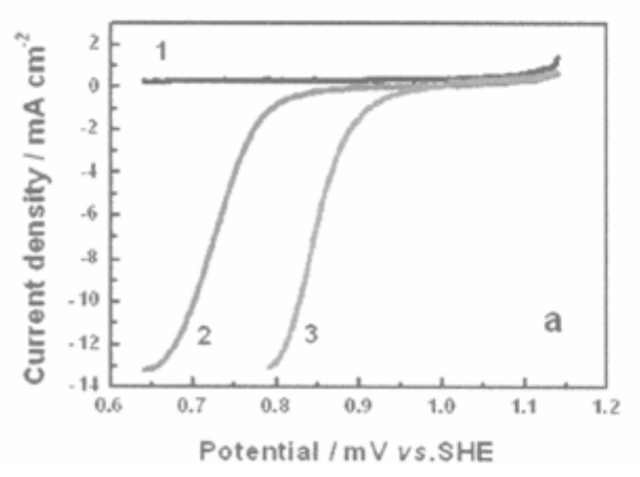
\includegraphics[scale = 0.5]{image227}
    \caption{Linear sweep curves of ORR in catalyst; W$_2$C, Pt/C, W$_2$C-Pt/C}
    \end{center}
\end{figure}
\end{frame}
% %%%%%%%%%%%%%%%%%%%%
\begin{frame}
\frametitle{ORR Catalyzed by Transition Metal Carbide}
\begin{figure}[htbp]
    \begin{center}
    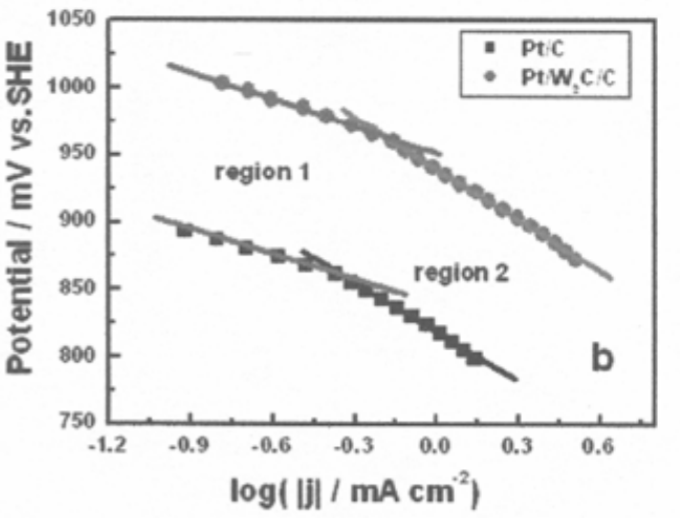
\includegraphics[scale = 0.5]{image228}
    \caption{Tafel Slopes of ORR on Pt/C and Pt-W$_2$C/C}
    \end{center}
\end{figure}
\begin{itemize}
\item{Has similar Tafel Slope with Pt/C: 66 mV/dec (low overpotential), 126 mV/dec (high overpotential)}
\item{Increased exchange current density of ORR: \newline
$(5.25 \times 10^{-10}, 3.15 \times 10^{-7}) \longrightarrow (4.7 \times 10^{-7}, 5.01 \times 10^{-5}) A/cm^2$}
\end{itemize}
\end{frame}



\end{document}
